% !TeX spellcheck = en_GB
\documentclass[../summary.tex]{subfiles}

\begin{document}
	
	\section{Food security}
	
	\subsection{Study guide}
	
	Students should understand \textbf{important concepts} such as food security, food gap, land gap, yield gap, the difference between synthetic and bio-based fertilizers, the difference between intensive and extensive farming, the difference between classic breeding technologies and genetically modified crops, plant protection products (PPP), integrated pest management (IPM), sustainable diet, protein shift, food waste and generational renewal.
	\\\\
	In addition, students should understand the \textbf{environmental impact of food production / agriculture} (land use, greenhouse gas emission, nutrient emission by synthetic fertilizers), including differences between animal-based versus plant-based foods.
	\\\\
	Finally, students should have insight into \textbf{solutions to increase food security} (increase yields, adopt healthy
	diets, reduce food waste)
	
	\subsection{Food security}
	
	Food security exists when all people, at all times, have physical and economic access to sufficient, safe and nutritious food that meets their dietary needs and food preferences for an active and healthy life. As we can see, this concept is very diverse. You can be food insecure because you simply can't afford to buy healthy food, but even if you're rich and have a lot of food available you can be food insecure because you eat unhealthy. 
	\\\\
	If we look at the evolution of famine deaths on figure \ref{fig:famine}, we can see that the number of famine mortality has decreased, even with the population growth of the last century. The main challenge of fighting hunger is currently situated in Africa. This has several causes such as climate change (resulting in yield losses), civil wars and anarchy. One of the goals of the United Nations is to end hunger, achieve food security and improved nutrition and promote sustainable agriculture by 2030. However, if we look at figure \ref{fig:undernourishment}, this is not very likely. One out of ten people worldwide are suffering from hunger and nearly one out of three people lack regular access to adequate food. Furthermore, rising food prices are affecting countries worldwide. Global crises like the climate crisis, the COVID-19  or the recent Ukraine crisis aren't really helping either.
	
	\begin{figure} [htbp]
		\centering
		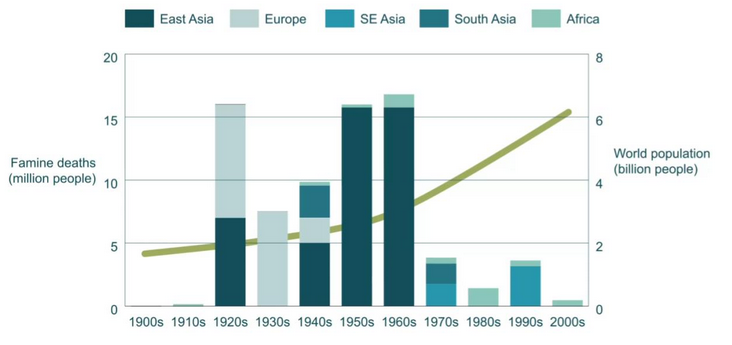
\includegraphics[width=1\linewidth]{images/6-famine.png}
		\caption{Evolution of famine deaths during 21st century}
		\label{fig:famine}
	\end{figure}
	
	\begin{figure} [htbp]
		\centering
		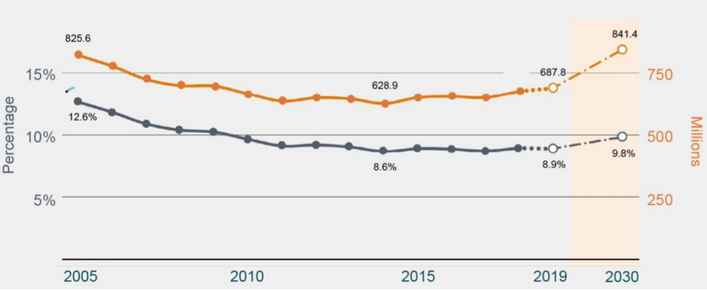
\includegraphics[width=1\linewidth]{images/6-undernourishment.png}
		\caption{Number of undernourished people (in percentage and in actual numbers)}
		\label{fig:undernourishment}
	\end{figure}
	
	As already established before, food security goes further then just hunger. We can distinguish between 3 faces of malnutrition when looking at the youngest generation: stunting, wasting and being overweight.
	\textbf{Stunting} means being too short for your age and \textbf{wasting} means being too thin for their height. The third face, being \textbf{overweight}, is something we see more and more in our own neighbourhoods. The challenge of fighting overconsumption, and hence also overweight and obesity, becomes the longer the more relevant. As a whole, there are more people overweight than underweight and the situation tends to get worse. Unhealthy food is often cheaper and more convenient than healthy food, but overweight leads to food related diseases, including for example obesity, type 2 diabetes, cardiovascular diseases and liver and kidney diseases. Overweight and obesity are measured with the BMI, body mass index. figure \ref{fig:obesity-and-caloric-intak} also shows there is a clear relationship between caloric intake per person on the one hand and the occurrence of overweight and obesity on the other hand.
	
	\begin{figure} [htbp]
		\centering
		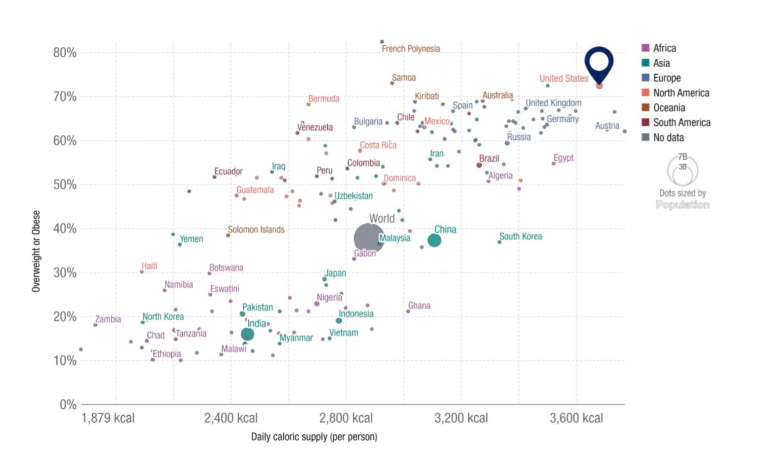
\includegraphics[width=0.9\linewidth]{images/6-obesity-and-caloric-intake.png}
		\caption{Relation between daily caloric intake and occurrence of overweight}
		\label{fig:obesity-and-caloric-intak}
	\end{figure}
	
	\subsection{Main challenges for food security}
	
	Two particularly important aspects to discuss whether or not we will we be able to produce enough food to feed the world population are the growing world population and the global surface area that can be allocated for food production. 
	\\\\
	The \textbf{food gap} measures how much food is needed to raise consumption at every income level to meet the minimum nutritional intake target per capita per day. Given the current population growth, we can expect a food gap of 56\% by 2050. In other words, where we needed about 13000 trillion calories to feed the world in 2010, we will need to produce over 20000 trillion calories by 2050. This is visualised on figure \ref{fig:food_gap}.
	
	\begin{figure}[htbp]
		\centering
		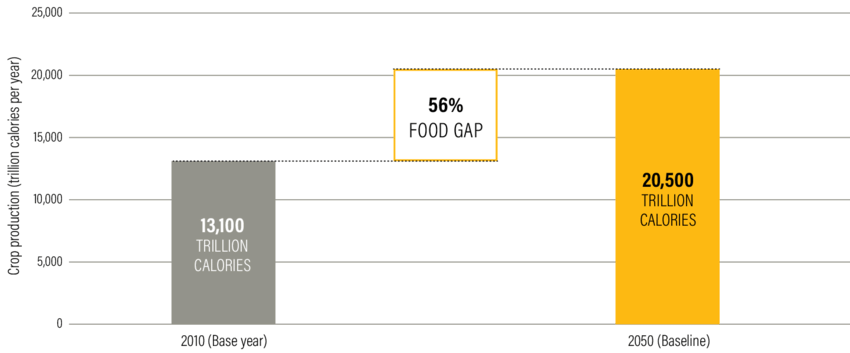
\includegraphics[width=1\linewidth]{images/6-food-gap.png}
		\caption{Food gap}
		\label{fig:food_gap}
	\end{figure}
	
	This food gap is also reflected in the \textbf{land gap}, which is the difference between the projected area of land needed to produce enough food in 2050 and the amount of agricultural land in 2010. On the left of figure \ref{fig:land_gap}, we can see that we need approximately 600 million ha of land extra to fill the food gap by 2050. This “business-as-usual scenario” considers the past trends in productivity gains we still have for our crop production system worldwide. However, in a second scenario where no productivity gains are taken into account, we need an extra 3200 million ha of agricultural land, this is more than 3 times the surface of the United States of America or almost all the land that is now covered by forests.
	\\
	\begin{figure}[htbp]
		\centering
		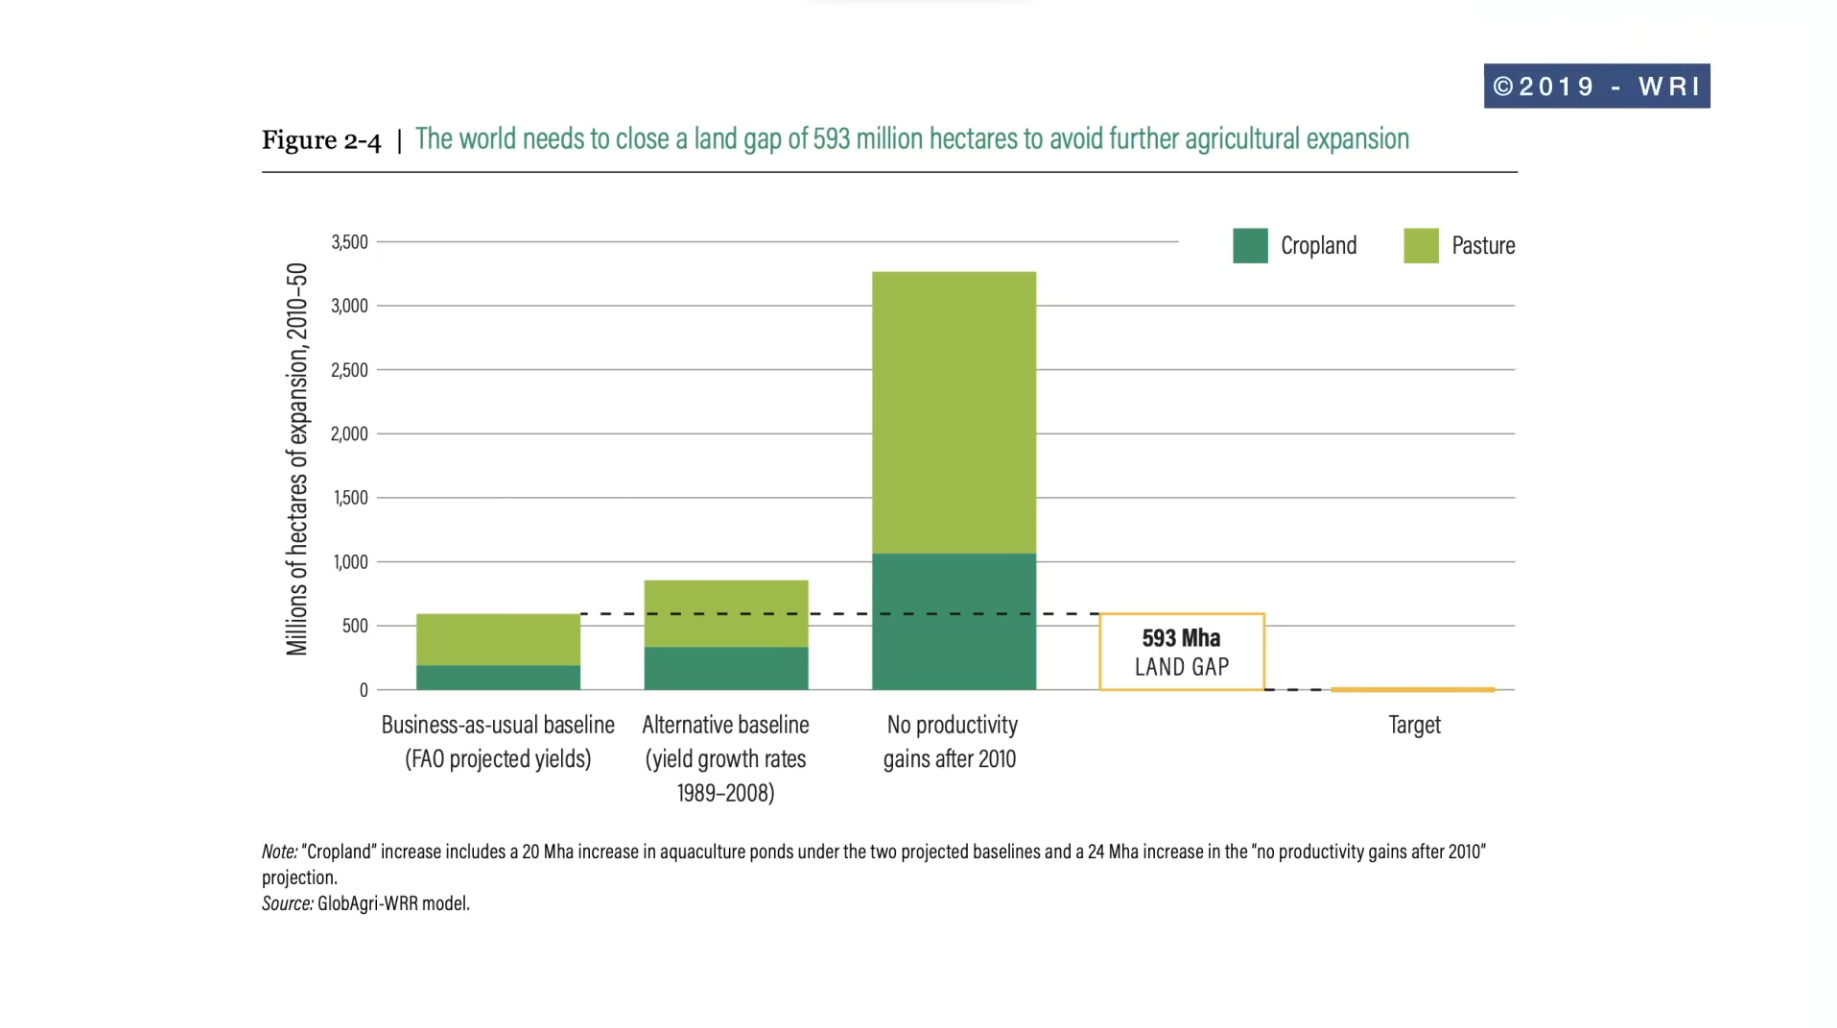
\includegraphics[width=1\linewidth]{images/6-land-gap.png}
		\caption{Land gap}
		\label{fig:land_gap}
	\end{figure}
	
	The \textbf{yield gap} represents the difference between the potential yield that could be achieved with optimal crop management practices and the actual yield obtained by farmers. This gap highlights the untapped potential for increasing production. Factors contributing to the yield gap include limited access to improved seeds, inadequate use of fertilizers and irrigation, pests and diseases and suboptimal agronomic practices. Addressing the yield gap requires targeted interventions, such as improving agricultural infrastructure, providing farmers with access to modern technologies and knowledge, promoting sustainable farming practices and supporting research and development efforts to develop high-yielding and resilient cereal varieties. By narrowing the yield gap, we can enhance global food security and contribute to the sustainable development of agriculture.
	\\\\
	A last big challenge for food security is \textbf{climate change}. The results of climate change currently already have an impact on yield and we expect this to continue, mostly in the global south.
	\newpage
	
	\subsection{Environmental impact of agriculture}
	
	Our food production system has a huge impact on the environment. There are four big environmental aspects that are influenced by agriculture and the food production system, namely land use, fresh water withdrawals, eutrophication and greenhouse gas emissions.
	\\\\
	Half of the world’s habitable land is used for agriculture. This \textbf{land use} has a serious impact on biodiversity. Changes in land use for agriculture and direct exploitation such as fishing, logging and hunting account for 50\% of the biodiversity losses. 
	\\\\
	The second impact is on \textbf{freshwater withdrawals}. 70\% of global freshwater withdrawals are used for agriculture. When we go more in detail on the water requirement per tonne of food product (figure \ref{fig:production-water-requirement}), we can conclude that the water requirement for the production of meat, especially beef, across the full supply chain is much higher than for most fruit, vegetables and arable crops.
	\\
	
	\begin{figure} [htbp]
		\centering
		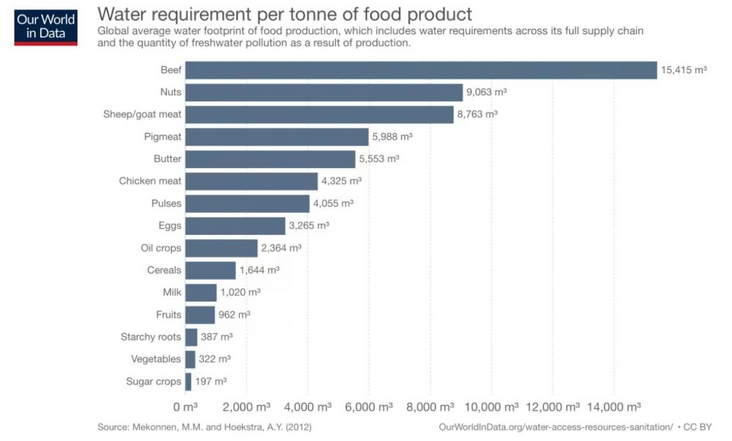
\includegraphics[width=1\linewidth]{images/6-product-water-requirement.png}
		\caption{Water requirement per ton of food product}
		\label{fig:production-water-requirement}
	\end{figure}
	
	The third aspect is \textbf{eutrophication}, which is the pollution of waterways with nutrient-rich water. 78\% of global ocean and freshwater eutrophication is caused by agriculture. This can be a result of the use of fertilizers such as nitrate and phosphate that can end up in rivers. This will lead to the overgrowth of algae in the water, which will lead to a lack of oxygen in the water, preventing other organisms to live. figure \ref{fig:result-of-fertilizers} showcases this.
	
	\begin{figure}[htbp]
		\centering
		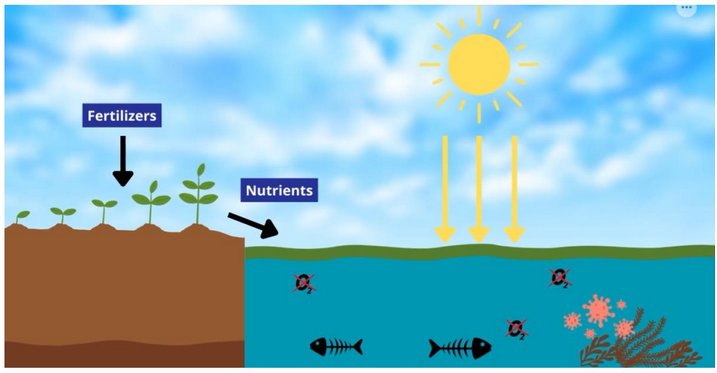
\includegraphics[width=1\linewidth]{images/6-result-of-fertilizers.png}
		\caption{Result of fertilizers}
		\label{fig:result-of-fertilizers}
	\end{figure}
	
	Finally, food production accounts for over a quarter of global \textbf{greenhouse gas emissions} and is a result of mainly livestock, crop production and land use. The total emission of greenhouses gasses including carbon dioxide or $CO_{2}$, methane or $CH_{4}$ and nitrous oxide or $N_{2}O$ also known as laughing gas, is at the moment approximately 52 gigaton  $CO_{2}$ equivalents per year. According to a study in 2018, 26\% of the greenhouse gas emissions are the result of our food production system. According to a study from 2021 this is even 34\%. When we now look a little bit more in detail and do not include land use change, we can see that (the production of methane in the digestive system of) livestock is responsible for approximately 40\% of the greenhouse gas emission within agriculture.
	
	\subsection{Sustainable food consumption}
	
	Making our food production more sustainable is a pressing global challenge that requires collective efforts and innovative solutions. With a growing population, increasing environmental concerns, and the need to ensure food security, sustainable food production practices are crucial. The most important interventions to reduce the impact of our food production system on the environment and safeguard food security are an increase of the yield, the adoption of healthy diets and a reduction of food waste and losses. 
	
	\subsubsection{Increasing yield to spare natural habitat}
	
	The first intervention is \textbf{increasing yield}. Intensification of crop production has been suggested as one of the promising strategies to reduce the amount of land used for agriculture. Interestingly, since 1961 1.75 billion hectares were spared due to crop yield improvements. In a recent study Folberth et al. showed that if we further optimize fertilizer use and distribute 16 major crops more efficiently across global croplands, we can reduce the amount of land needed to maintain current levels of production by nearly 50\%.
	
	\subsubsection{Key strategies for developing nations}
	
	Although a context-specific approach is necessary, there are some key strategies to increase the yield for developing nations. Some strategies, related to the production systems are summarized below:
	
	\begin{itemize}
		\item Access to improved inputs such as high-quality seeds, fertilizers, and efficient low-risk pesticides.
		\item Strengthening agricultural extension services and promoting the transfer of knowledge and innovative technologies to farmers. This includes providing training on best farming practices, crop management techniques, and the use of modern tools and machinery.
		\item Efficient irrigation methods, such as drip irrigation and precision water management, should be promoted to optimize water use and minimize wastage.
		\item Promoting sustainable soil management practices, can improve soil health and fertility. This involves practices like crop rotation, organic matter incorporation, and balanced nutrient application, tailored to the specific conditions of each region.
		\item Encouraging climate-smart agricultural practices that promote resilience to climate change is crucial. 	
	\end{itemize}
	
	\subsubsection{Intensive versus extensive farming}
	
	Furthermore, we can also make a distinction between intensive and extensive farming. In \textbf{intensive farming}, fertilizers, crop protection products and monocultures are used. Intensive farming is also often referred to as conventional farming and leads to high yields but lower biodiversity. In \textbf{extensive or organic farming} on the other hand, no synthetic crop protection products, synthetic fertilizers or genetically modified plants can be used. This type of farming results in lower yields but higher biodiversity. Based on a metastudy it can be concluded that, depending on the crop as well as the region and environmental conditions, we can have yield reductions in organic farming compared to conventional farming between 19 to 25\%. However, when we look at biodiversity, depending on the species groups, we see increases in the number of species between 1 to 38\% and an increase in the total number of organisms between 40-50\% compared to conventional farming. Therefore we need to make intensive farming more sustainable so that we can produce more on less land, freeing up space for nature.
	
	\newpage
	\subsubsection{Sustainable crop breading}
	
	The next subject we can study, is \textbf{sustainable crop breading}. Classic breeding technologies, such as selective breeding and hybridization, have been employed for centuries to improve crop traits such as yield, disease resistance, and drought tolerance. These traditional breeding methods rely on natural genetic variation within a crop species and involve crossing plants with desired traits to generate offspring with improved characteristics. In recent decades, genetically modified (GM) crops have emerged as a powerful tool in crop breeding. GM crops are engineered to possess specific genes from the same species (different variety; cis-genesis) or other organisms (trans-genesis), offering the potential to introduce desired traits more rapidly and precisely. These traits can include enhanced pest resistance, tolerance to herbicides, and increased nutritional value. Another emerging technology with significant potential is genome editing (“new breeding technology”), which allows for targeted modifications of specific genes within an organism's genome. Techniques such as CRISPR-Cas9 have revolutionized the field of genetic engineering, enabling more precise and efficient genetic modifications in crops. 
	
	\subsubsection{Plant protection}
	
	Global crop production is threatened by various diseases and pests caused by for example fungi, viruses, bacteria and insects. Globally, these diseases and pests still cause up to 20-30\% production losses. 
	\\\\
	\textbf{Plant protection products or PPPs} are used to control these diseases and pests. By definition, these are products that protect plants or plant products during production and storage from pests. Often the terminology "pesticides" is used, but the terminology “PPP” is more correct. The main PPP are insecticides, fungicides and herbicides. They control insects, fungi and weeds, respectively. The use of PPPs can have adverse effects on the environment and humans. For example, certain PPPs can also have an effect on non-target organisms such as pollinators. Moreover, through frequent and improper use resistance to these PPPs can occur. 
	\\\\
	An impact study performed by the University of Wageningen calculated that yield reductions will occur when we reduce PPPs, especially for crops such as apples, tomatoes, grapes and olives. In addition, we will have to import more crops and there will be declines in net exports, both of which will have significant economic impacts. We therefore will have to be very careful and focus on further sustainably optimizing our crop production systems and engage in agricultural innovations. First, we must strive for a better implementation and follow-up of \textbf{integrated pest management (IPM)}. IPM consists of five steps.
	
	\begin{enumerate}
		\item \textbf{ Knowledge}: as a farmer you need to know which pests can harm your crop under which conditions and when.
		\item \textbf{Prevention} of harmful organisms can be achieved by e.g. choosing cultivar that are more resistant to the pest, by implementing crop rotation avoiding build up of your pest inoculum or by hygiene measures e.g. regular cleaning of machinery and equipment.
		\item \textbf{Monitoring}: Harmful organisms must be monitored. Adequate tools for monitoring could include observations in the field as well as scientifically sound warning, forecasting and early diagnosis systems.
		\item \textbf{Intervention}: Based on the results of the monitoring the farmer has to decide whether and when to intervene. Sustainable biological and mechanical methods must be preferred to chemical PPPs but only if they provide satisfactory pest control.
		\item \textbf{Evaluation and planning}: The farmer should evaluate the problems he encountered and the interventions he performed in order to optimize the plan for the next season. 
	\end{enumerate}
	
	\newpage
	\subsubsection{Sustainable food consumption}
	
	A more sustainable food system has many aspects, including sustainable consumption. It is important to note that sustainable food, as such, doesn’t exist. To evaluate someone’s consumption behavior, you need to look at his or her entire food diet, not just at a single product. Evaluating the sustainability of your diet, one can identify three aspects: health, ecology and social aspects related to food production.
	\\\\
	Let’s start with the \textbf{health} component. At the global level, almost 10\% of the adult population is underweight and over 30\% is overweight or obese. While underweight is especially an issue in the global South, overweight occurs in the North as well as in the South. This often goes paired with diseases like diabetes type 2 for example. This clearly demonstrates that we need to invest in promoting healthy diets if we want to strive for sustainable food consumption.
	\\\\
	The second component of sustainable food consumption is \textbf{environment}. The number of labels claiming environmental friendly food is endless. But if we look at the data on GHG emissions of our food system in Figure \ref{fig:greenhouse-gas}, it becomes clear that it is most relevant to focus on what is on your plate, rather than to focus on how your food is produced, where it comes from, how it is processed or packed because the majority of the footprint of food relates to landuse and agriculture. 
	
	\begin{figure} [htbp]
		\centering
		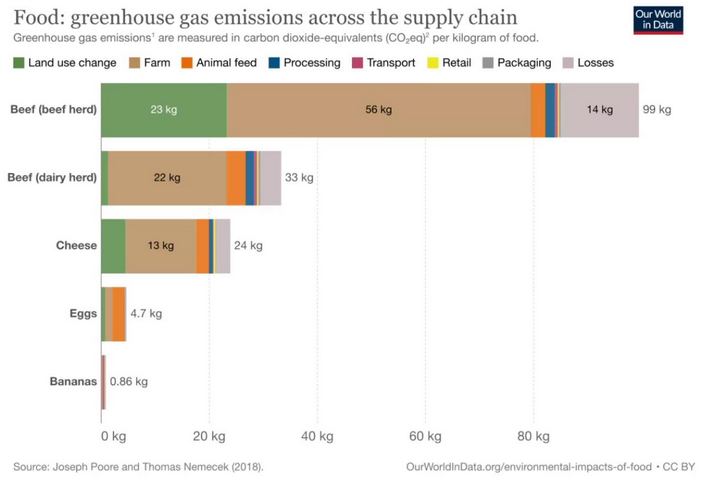
\includegraphics[width=1\linewidth]{images/6-greenhouse-gas.png}
		\caption{Greenhouse gas emissions of food across the supply chain}
		\label{fig:greenhouse-gas}
	\end{figure}
	
	Overall, a better balance between animal and plant based products in our diets, contribute significantly to lowering our footprint. A \textbf{protein shift}, where you move from a meat based diet to a plant based diet, is not just more healthy, it is also better for the environment. 
	\\\\
	The third aspect of sustainable food consumption has to do with \textbf{social and economic aspects}. The power in the food system is very badly balanced, with farmers being the weakest actor in the food chain. Fair trade labels have been introduced as a tool to develop more ‘fair’ food systems. 
	
	\subsubsection{Food waste}
	
	 \textbf{Food waste} is defined as food and the associated inedible parts removed from the human food supply chain in the sectors of retail, food service and households. In this definition, “removed from the human food supply chain” means one of the following end destinations: landfill, controlled combustion, sewer, litter/discards/refuse, co/anaerobic digestion, compost/aerobic digestion or land application. Food itself is defined as any substance – whether processed, semi-processed or raw – that is intended for human consumption. Therefore, food waste includes both edible parts (i.e., the parts of food that were intended for human consumption) and inedible parts (components associated with a food that are not intended to be consumed by humans). 
	 \\\\
	 Food waste reduction offers multi-faceted wins for people and planet, improving food security, addressing climate change, saving money and reducing pressures on land, water, biodiversity and waste management systems. 
	 
\end{document}